\documentclass{article}
\usepackage{physics}
\usepackage{siunitx}
\usepackage{graphicx}
\usepackage{courier}
\usepackage{listings}
\usepackage{amsmath}

\title{NE583 Test 2}
\author{J.R. Powers-Luhn}
\date{November 20, 2018}

\begin{document}

\maketitle

\section{Problem 1}

\subsection{$^{238}$U}

Calculate total cross section

\[
\sigma_t = \SI{5}{\barn} + 
\begin{cases}
	0, & \text{if } E < \SI{6.52}{\electronvolt} \text{ or } E > \SI{6.62}{\electronvolt} \\
	160000 \times (E - \SI{6.52}{\electronvolt}), & \text{if } \SI{6.52}{\electronvolt} < E < \SI{6.57}{\electronvolt} \\
	160000 \times (\SI{6.62}{\electronvolt} - E), & \text{if } \SI{6.57}{\electronvolt} < E < \SI{6.62}{\electronvolt}
\end{cases}
\]

Calculate flux scaling

\[
f = \int_6^7 \frac{\dd{E}}{E \sigma_t} = 0.0277995
\]

Calculate group cross section

\[
	\int_6^7 \dd{E} \frac{\sigma_t \psi(E)}{f E} = \int_6^7 \dd{E} \frac{\sigma_t}{f E^2 \sigma_t} = \frac{1}{f}\left( \frac{1}{6} - \frac{1}{7}\right) = \SI{0.8565}{\barn}
\]

\subsection{H}

Calculate flux scaling

\[
f = \int_6^7 \frac{\dd{E}}{E \sigma_t} = \frac{1}{20} \ln \frac{7}{6} = 0.007708
\]

Calculate group cross section

\[
\frac{1}{f} \int_6^7 \dd{E} \frac{\sigma_t}{E^2 \sigma_t} = \SI{3.089}{\barn}
\]

\subsection{50/50 Mix of U and H}

\[
	\sigma_t = 0.5 \sigma_t^H + 0.5 \sigma_t^U
\]

Plug this in to the flux equation and integrate to get a scaling factor of $f=0.011136$. Then integrate (numerically) to get $\sigma_t = \SI{2.1380}{\barn}$.

\pagebreak
\section{Problem 2}

\subsection{Normalization factor}

\begin{align*}
\int_6^7 \psi(E) \dd{E} &= \int_6^7 \frac{1}{E} \dd{E} \\
&= \log{7} - \log{6} \\
f &= 0.154151
\end{align*}

\subsection{Alpha}

\begin{align*}
\alpha = \frac{(A-1)^2}{(A+1)^2} = 0
\end{align*}

\subsection{Scattering Cross section}

\begin{align*}
\sigma_s^{gg} &= \int_6^7 \dd{E^\prime} \int_{E^\prime}^7 \dd{E} \frac{\sigma}{(1 - \alpha)E} \frac{\psi(E)}{f} \\
&= \frac{\sigma}{f} \int_6^7 \dd{E^\prime} \int_{E^\prime}^7 \frac{\dd{E}}{E^2} \\
&= \frac{\sigma}{f} \int_6^7 \dd{E^\prime} \left( \frac{-1}{7} - \frac{-1}{{E^\prime}} \right) \\
&= \frac{\sigma}{f} \left( \int_6^7 \frac{\dd{E^\prime}}{{E^\prime}} - \int_6^7 \frac{\dd{E^\prime}}{7} \right) \\
&= \frac{\SI{20}{\barn}}{0.154151} \left( \ln \frac{7}{6} - \frac{1}{7} \right) \\
&= \SI{1.46526}{\barn}
\end{align*}

\pagebreak
\section{Problem 3}

	%\lstinputlisting[language=python]{"Problem 3.py"}
	%\input{"Problem 3.tex"}

\section{Problem 4}

\pagebreak
\section{Problem 5}

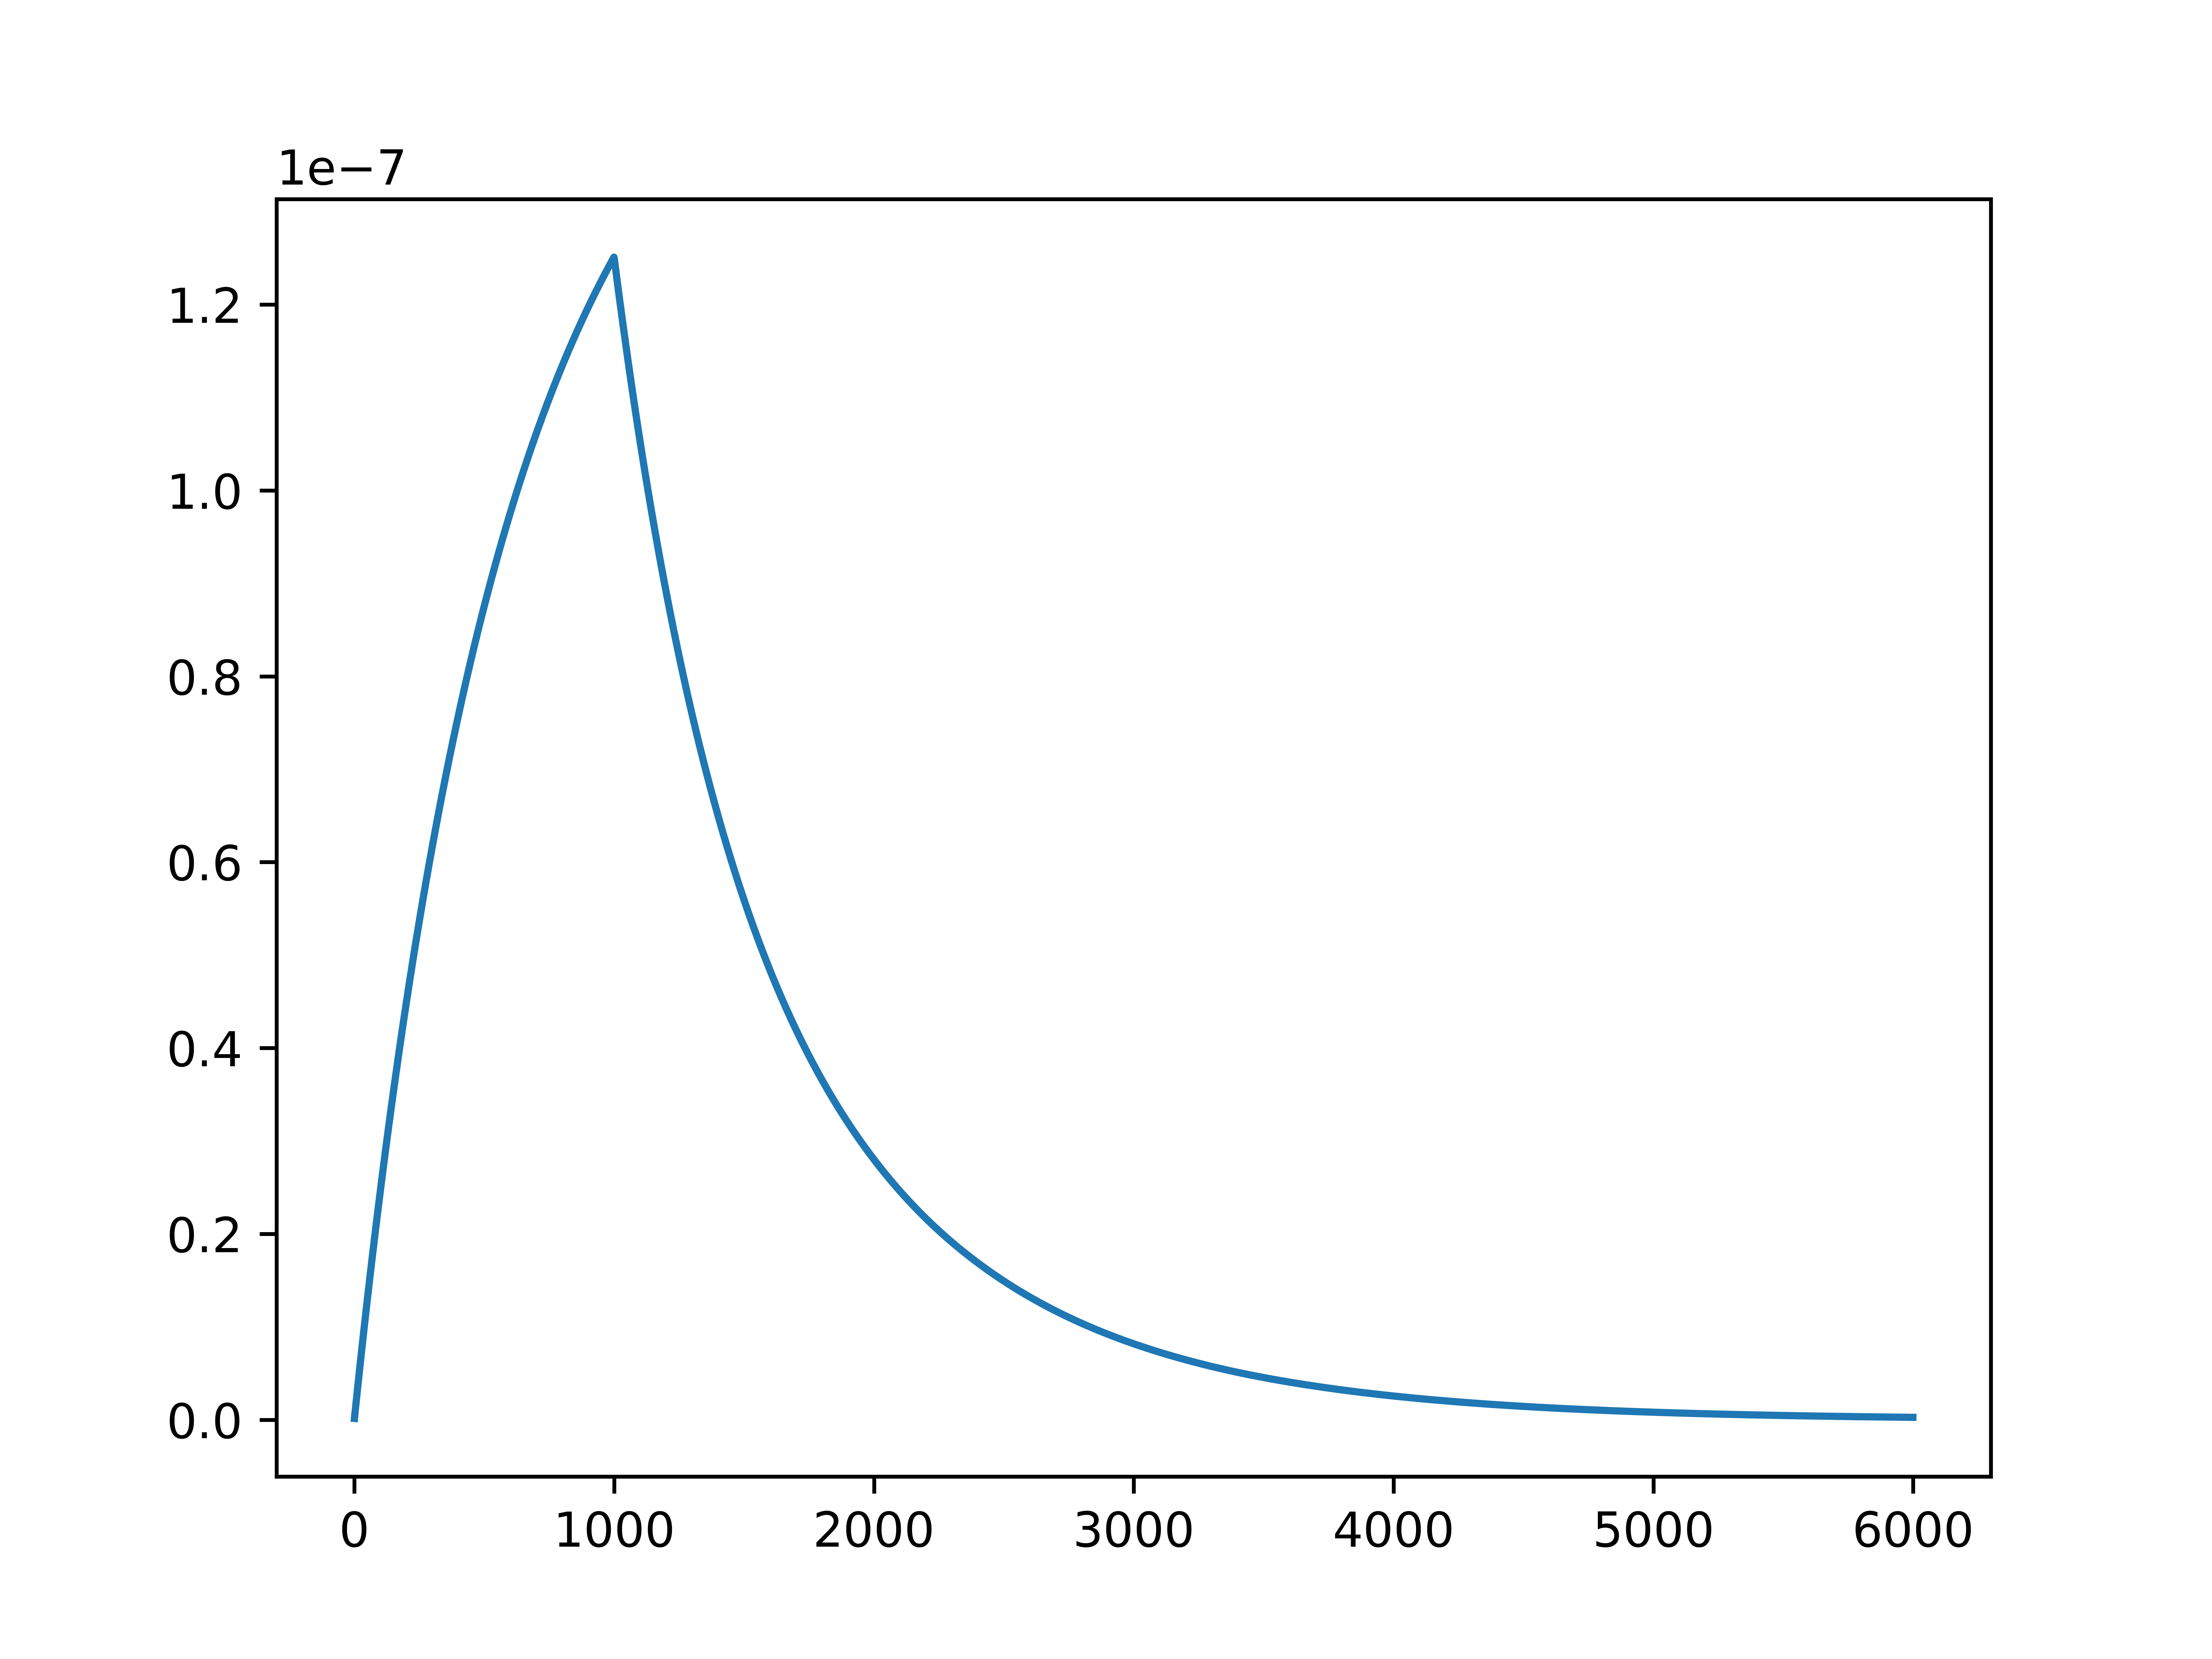
\includegraphics[width=\textwidth]{no5result}

The orange line in the graph above was calculated using the code in the file \texttt{test2no5.java} (reproduced below). It 
is compared with the pseudo-analytic curve (blue line) which was generated by calculating the 
distance from every point in the source region to every point in the top row (in units of mean free 
paths) and assuming $\mathrm{e^{-r}}$ absorption and $\frac{1}{r^2}$ spatial falloff.

The quadrature solution shows a much more peaked distribution as a result of ray effects.

\lstinputlisting[language=java]{"test2no5.java"}

\end{document}